

% sldies for T-61.6080 special course in bioinformatics 2, Spring 2015
\documentclass[first=dgreen,second=purple,logo=yellowexc]{aaltoslides}

% macro


% input encode
\usepackage[utf8]{inputenc}


%\usepackage[T1]{fontenc}
%\usepackage{lastpage}
%\usepackage{multirow}
%\usepackage{colortbl}
%\usepackage{comment}
%\usepackage{bm}
%\usepackage{natbib}


% Lipsum package generates bullshit
%\usepackage{lipsum}

% Set the document languages
%\usepackage[finnish,swedish,english]{babel}

% nomenclature
%\usepackage[intoc]{nomencl}

% math
\usepackage{amsmath}

% bibliograph
%\usepackage{natbib}

% For algorithms
\usepackage{algorithm}
\usepackage{algorithmic}

% math font
\usepackage{amsfonts}

% theory
%\usepackage{amsthm}

% double bracket
\usepackage{stmaryrd}

% special math symbol
\usepackage{amssymb}

% use enumerate environment
%\usepackage{enumitem}

% use \url \hyperref, make reference clickable
\usepackage{hyperref}

% use lastpage to inde
\usepackage{lastpage}



%-------------------
%
% set
%
%-------------------
\newcommand{\Acal}{\mathcal{A}}
\newcommand{\Bcal}{\mathcal{B}}
\newcommand{\Ccal}{\mathcal{C}}
\newcommand{\Dcal}{\mathcal{D}}
\newcommand{\Ecal}{\mathcal{E}}
\newcommand{\Fcal}{\mathcal{F}}
\newcommand{\Gcal}{\mathcal{G}}
\newcommand{\Hcal}{\mathcal{H}}
\newcommand{\Ical}{\mathcal{I}}
\newcommand{\Jcal}{\mathcal{J}}
\newcommand{\Kcal}{\mathcal{K}}
\newcommand{\Lcal}{\mathcal{L}}
\newcommand{\Mcal}{\mathcal{M}}
\newcommand{\Ncal}{\mathcal{N}}
\newcommand{\Ocal}{\mathcal{O}}
\newcommand{\Pcal}{\mathcal{P}}
\newcommand{\Qcal}{\mathcal{Q}}
\newcommand{\Rcal}{\mathcal{R}}
\newcommand{\Scal}{\mathcal{S}}
\newcommand{\Tcal}{\mathcal{T}}
\newcommand{\Ucal}{\mathcal{U}}
\newcommand{\Vcal}{\mathcal{V}}
\newcommand{\Wcal}{\mathcal{W}}
\newcommand{\Xcal}{\mathcal{X}}
\newcommand{\Ycal}{\mathcal{Y}}
\newcommand{\Zcal}{\mathcal{Z}}

\newcommand{\RR}{\mathbb{R}}
\newcommand{\ZZ}{\mathbb{Z}}

%-------------------
%
% vector
%
%-------------------
\newcommand{\va}{\mathbf {a}}
\newcommand{\vb}{\mathbf {b}}
\newcommand{\vc}{\mathbf {c}}
\newcommand{\vd}{\mathbf {d}}
\newcommand{\ve}{\mathbf {e}}
\newcommand{\vf}{\mathbf {f}}
\newcommand{\vg}{\mathbf {g}}
\newcommand{\vh}{\mathbf {h}}
\newcommand{\vi}{\mathbf {i}}
\newcommand{\vj}{\mathbf {j}}
\newcommand{\vk}{\mathbf {k}}
\newcommand{\vl}{\mathbf {l}}
\newcommand{\vm}{\mathbf {m}}
\newcommand{\vn}{\mathbf {n}}
\newcommand{\vo}{\mathbf {o}}
\newcommand{\vp}{\mathbf {p}}
\newcommand{\vq}{\mathbf {q}}
\newcommand{\vr}{\mathbf {r}}
\newcommand{\vs}{\mathbf {s}}
\newcommand{\vt}{\mathbf {t}}
\newcommand{\vu}{\mathbf {u}}
\newcommand{\vv}{\mathbf {v}}
\newcommand{\vw}{\mathbf {w}}
\newcommand{\vx}{\mathbf {x}}
\newcommand{\vy}{\mathbf {y}}
\newcommand{\vz}{\mathbf {z}}
\newcommand{\vmu}{\mathbf {\mu}}
\newcommand{\valpha}{\mathbf {\alpha}}
\newcommand{\vlambda}{\mathbf {\lambda}}
\newcommand{\vAlpha}{\mathbf {\Alpha}}
\newcommand{\vbeta}{\mathbf {\beta}}
\newcommand{\vBeta}{\mathbf {\Beta}}
\newcommand{\vgamma}{\mathbf {\gamma}}
\newcommand{\vGamma}{\mathbf {\Gamma}}
\newcommand{\vdelta}{\mathbf {\dalta}}
\newcommand{\vDelta}{\mathbf {\Dalta}}
\newcommand{\vone}{\mathbf {1}}
\newcommand{\vzero}{\mathbf {0}}
\newcommand{\vell}{\mathbf {\ell}}
\newcommand{\vxi}{\mathbf{\xi}}
\newcommand{\vphi}{\mathbf{\phi}}
\newcommand{\vPhi}{\mathbf{\Phi}}

%-------------------
%
% math operation
%
%-------------------
\newcommand{\argmax}{\textbf{argmax}}
\newcommand{\argmin}{\textbf{argmin}}
\newcommand{\sign}{\textbf{sign}}
\newcommand{\maximize}{\textbf{max}}
\newcommand{\minimize}{\textbf{min}}
\newcommand{\argkmax}{\textbf{argkmax}}
\newcommand{\argkmin}{\textbf{argkmin}}
\newcommand{\kmaximize}{\textbf{kmax}}
\newcommand{\kminimize}{\textbf{kmin}}
\newcommand{\st}{\textbf{s.t.}}
\newcommand{\set}[1]{\{ #1 \}}
%\newcommand{\ind}[1]{{\llbracket #1 \rrbracket}}
\newcommand{\ind}[1]{\mathbf{1}_{\{#1\}}}
\newcommand{\norm}[1]{\left|\left| #1 \right|\right|}
\newcommand{\ip}[2]{\langle #1, #2 \rangle}
\newcommand{\var}{\textbf{Var}}
\newcommand{\E}{\textbf{E}}
\newcommand{\exponential}[1]{e^{ #1 }}


\newcommand{\Gva}{G_{\va}}
%-------------------
%
% writings
%
%-------------------
\newcommand{\eqdef}{\overset{{\rm \mbox{\tiny def}}}{=}}
\newcommand{\sbf}[1]{\boldsymbol{#1}}
\newcommand{\mbf}[1]{\mathbf{#1}} 
\newcommand{\etal}{{\em et al.}}

\newcommand{\svmstruct}{{\sc ssvm}}
\newcommand{\mmmn}{{\sc m$^3$n}}
\newcommand{\svm}{{\sc svm}}
\newcommand{\mmcrf}{{\sc mmcrf}}
\newcommand{\smo}{{\sc smo}}
\newcommand{\crf}{{\sc crf}}
\newcommand{\nphard}{$\Ncal\Pcal$-hard}
\newcommand{\nphardness}{$\Ncal\Pcal$-hardness}
\newcommand{\iis}{{\sc iis}}
\newcommand{\memm}{{\sc memm}}
\newcommand{\lr}{{\sc lr}}
\newcommand{\svmlight}{{\sc svmlight}}
\newcommand{\libsvm}{{\sc libsvm}}
\newcommand{\svmcascade}{{\sc svmcascade}}
\newcommand{\adaboost}{{\sc adaboost}}
\newcommand{\adaboostmh}{{\sc adaboost.mh}}
\newcommand{\bagging}{{\sc bagging}}
\newcommand{\vrtree}{{\sc vr-tree}}
\newcommand{\deepboosting}{{\sc deepboosting}}
\newcommand{\loo}{{\sc loo}}
\newcommand{\mtl}{{\sc mtl}}
\newcommand{\sdp}{{\sc sdp}}
\newcommand{\iqp}{{\sc iqp}}
\newcommand{\qp}{{\sc qp}}
\newcommand{\daggraph}{{\sc dag}}
\newcommand{\lp}{{\sc lp}}

\newcommand{\hatf}{{\hat{f}}}
\newcommand{\p}{\sc p}
\newcommand{\n}{\sc n}
\newcommand{\pp}{\sc pp}
\newcommand{\pn}{\sc pn}
\newcommand{\nn}{\sc nn}
\newcommand{\maxcut}{{\sc max-cut}}
\newcommand{\greedy}{{\sc greedy}}
\newcommand{\kernelcascade}{{\sc kernel cascade}}
\newcommand{\netrate}{{\sc netrate}}
\newcommand{\netinf}{{\sc netinf}}
\newcommand{\spin}{{\sc spin}}
\newcommand{\vI}{\mathbf{I}}
\newcommand{\tp}{^{\intercal}}
\newcommand{\mve}{{\sc mve}}
\newcommand{\amm}{{\sc amm}}
\newcommand{\mam}{{\sc mam}}
\newcommand{\rta}{{\sc rta}}
\newcommand{\lasso}{{\sc lasso}}
\newcommand{\mle}{{\sc mle}}
\newcommand{\map}{{\sc map}}
\newcommand{\rbf}{{\sc rbf}}
\newcommand{\mlknn}{{\sc ml-knn}}
\newcommand{\knn}{{\sc knn}}
\newcommand{\iblr}{{\sc iblr}}
\newcommand{\cc}{{\sc cc}}
\newcommand{\pcc}{{\sc pcc}}
\newcommand{\ecc}{{\sc ecc}}
\newcommand{\br}{{\sc br}}
\newcommand{\corrlog}{{\sc corrlog}}
\newcommand{\ilgs}{{\sc ilgs}}
\newcommand{\ilrs}{{\sc ilrs}}
\newcommand{\cpp}{{\sc c}}
\newcommand{\matlab}{{\sc matlab}}
\newcommand{\openmp}{{\sc openmp}}
\newcommand{\python}{{\sc python}}
\newcommand{\cvx}{{\sc cvx}}
\newcommand{\lda}{{\sc lda}}
\newcommand{\kkt}{{\sc k.k.t}}
\newcommand{\lbp}{{\sc lbp}}
\newcommand{\anova}{{\sc anova}}

\renewcommand{\algorithmicrequire}{\textbf{Input:}}
\renewcommand{\algorithmicensure}{\textbf{Output:}}



\newcommand{\Upsilonb}{\pmb \Upsilon}
\newcommand{\phib}{\pmb \phi}
\newcommand{\psib}{\pmb \psi}
\newcommand{\varphib}{\pmb \varphi}
\newcommand{\phibh}{\hat\phib}
\newcommand{\psibh}{\hat \psib}
\newcommand{\vYcal}{\pmb \Ycal}
\newcommand{\vXcal}{\pmb \Xcal}
\newcommand{\vFcal}{\pmb \Fcal}
%-------------------
%
% others
%
%-------------------




%\newtheorem{definition}{Definition}
%\newtheorem{theory}{Theory}
%\newtheorem{lemma}{Lemma}














% title and other informtions
\title{Molecular classification}
\subtitle{T-61.6080 Special Course in Bioinformatics}
\author[H. Su]{Hongyu Su}
\institute[ICS]{Department of Information and Computer Science\\Aalto University, School of Science and Technology\\hongyu.su@aalto.fi}
\aaltofootertext{Classification learning (H.Su)}{\today}{\arabic{page}/\pageref{LastPage}\ }

%\date{Version 1.0, \today}
\date{ \today}
\AtBeginSection[]
{
  \begin{frame}<beamer>{Outline}
    \tableofcontents[currentsection,subsection]
  \end{frame}
}

% start the main contain of the document
\begin{document}


\aaltotitleframe



\footnotesize{


\begin{frame}{Content}
	\begin{itemize}
		\item Learning for classification
		\begin{itemize}
			\footnotesize
			\item Statistic learning
			\item Empirical risk minimization
			\item Regularization
			\item Support vector machines for single-task classification
			\item Kernel methods 
		\end{itemize}
		\item Molecular classification problem
		\begin{itemize}
			\footnotesize
			\item Predicting anti-cancer potentials of molecules
			\item Hierarchical molecule classification
		\end{itemize}
		\item Multi-task classification
		\begin{itemize}
			\item 
		\end{itemize}
	\end{itemize}
\end{frame}
\begin{frame}{Learning for classification}{Example: dog vs. cat?}
	\begin{itemize}
		\item We have $5000$ pictures of dog and $5000$ pictures of cat.
		\begin{center}
			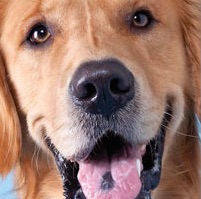
\includegraphics[scale=0.3]{./figures/dog.jpg}
			\text{     }
			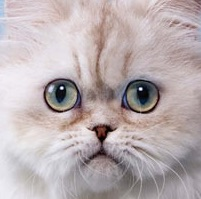
\includegraphics[scale=0.3]{./figures/cat.jpg}
		\end{center}
		\item Each picture is digitalized into $100\times100$ pixels, $\vx \in R^{10000}$.
		\item Given a new picture, we want to answer: is it a dog or a cat?
		\item This is a Kaggle competition (https://www.kaggle.com/c/dogs-vs-cats)
		\item The idea is to test the CAPTCHA system is safe from machine learning attack.
		\item Simple for human, dog, or cat. It used to be difficult for machines, with $82.7\%$ accuracy \citep{Golle08machine} before competition and $98.9\%$ afterwards.
	\end{itemize}
\end{frame}

\begin{frame}{Statistical learning}
	\begin{itemize}
		\item Two random variable $\vx\in\vXcal$ and $y\in\Ycal$ are jointly distributed according to some fixed but unknown distribution $P(\vx,y)$.
		\item $\vXcal=\RR^d$ is an input (instance) space, and $\Ycal=\{-1,+1\}$ is an output (label) space.
		\item Examples are given in pair $(\vx,y)\in\vXcal\times\Ycal$ generated by sampling from distribution $P(\vx,y)$.
		\item A hypothesis class $\Hcal$ is a set of function to be explored, for example, a set of hyperplanes in the feature space $f(\vx)=\ip{\vw}{\vx}+b=0, \vw\in\RR^d$. 
		\item The goal of statistical learning is to provide an estimator $f\in\Hcal:\vXcal\rightarrow\Ycal$ that predicts the best output $y$ for an input $\vx$. 
	\end{itemize}
\end{frame}


\begin{frame}{Loss function}
	\begin{itemize}
		\item Loss function measures the goodness of an estimator $f(\vx)$ on a single training example $(\vx_i,y_i)$
		\begin{align*}
			\ell(f(\vx_i),y_i):\Ycal\times\Ycal\rightarrow\RR^+.
		\end{align*}
		\item It is a monotonic bounded function defined on an estimation and the ground truth.
		\item The simplest one is hamming loss, which return $1$ if the estimation is the same as the ground truth, $0$ otherwise.
		\begin{align*}
			\ell_{hamming}(f(\vx_i),y_i) = \ind{\vy_i=f(\vx_i)}
		\end{align*}
		\item Many other loss functions: {hinge loss} in support vector machines \citep{Cortes95support}, {$0/1$ loss} in structured \svm\ \citep{THJA04}, {squared loss} in ridge regression \citep{Hoerl00ridge}, {exponential loss} in \adaboost\ \citep{Schapire99improved}, {logistic loss} in logistic regression \citep{Chen99}.
	\end{itemize}
\end{frame}


\begin{frame}{Empirical risk minimization}
	\begin{itemize}
		\item In the end, we want to minimize the true risk of an estimator over a domain $\vXcal\times\Ycal$
		\begin{align*}
			R_{true}(f) = \int_{(\vx,y)\in\vXcal\times\Ycal}\ell(y,f(\vx))P(\vx,y)\,d_{\vx}d_{y}. \quad\text{\color{aaltoblue} Test error}
		\end{align*}
		\item It is impossible to compute the true risk directly, as $P(\vXcal, \Ycal)$ is known.
		\item We are given a set of $m$ training examples $\Scal=\{(\vx_i,y_i)\}_{i=1}^{m}$.
		\item The empirical risk of an estimator $f\in\Hcal$ over $\Scal$ is
		\begin{align*}
			R_{emp}(f) = \frac{1}{m}\sum_{i=1}^m\ell(y_i,f(\vx_i)). \quad\text{\color{aaltoblue} Training error}
		\end{align*}
		\item Empirical risk minimization strategy \citep{Vapnik92principles} suggests we should search for an estimator that minimizes the empirical risk with regards to the training data.
		\item \citet{Vapnik92principles} showed that true risk is upper bounded by empirical risk
		\begin{align*}
			R_{true}(f) \le R_{emp}(f) + \sqrt{\frac{h(\log(\frac{2m}{h}+1)-\log(\frac{\eta}{4}))}{m}}.
		\end{align*}
	\end{itemize}
\end{frame}


\begin{frame}{Empirical risk minimization}{An example}
	\begin{itemize}
		\item Training examples from two classes are located in $2$ dimensional space.
		\item We are searching for a linear function (hyperplane) to separate two classes.
		\item Empirical minimization principle is applied.
		\begin{center}
			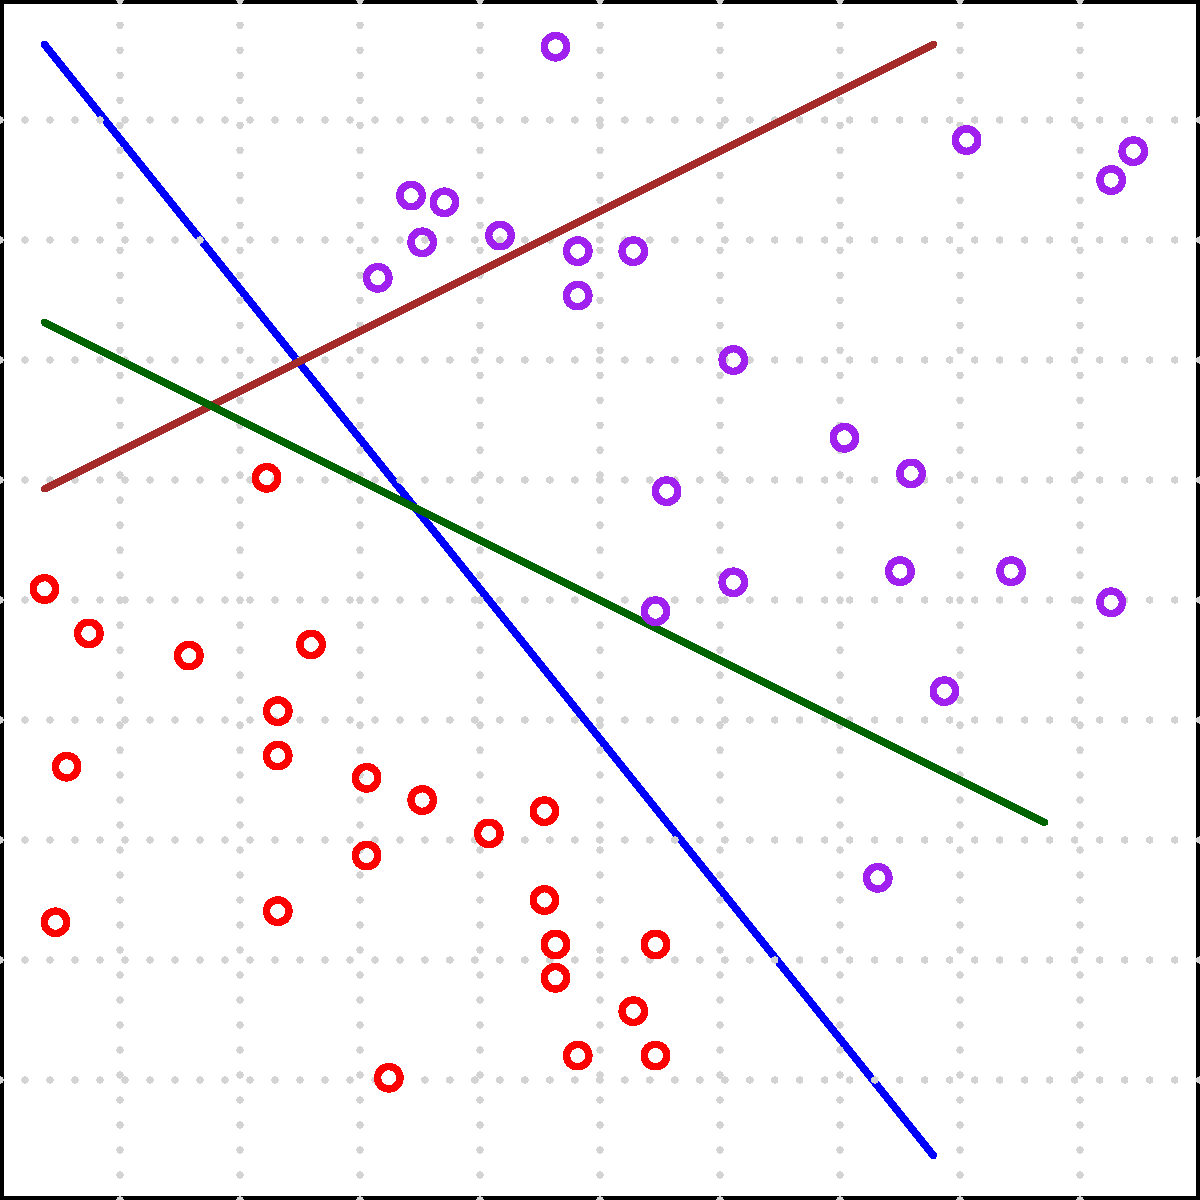
\includegraphics[scale=0.1]{./figures/empirical_risk_1.pdf}
			\text{      }
			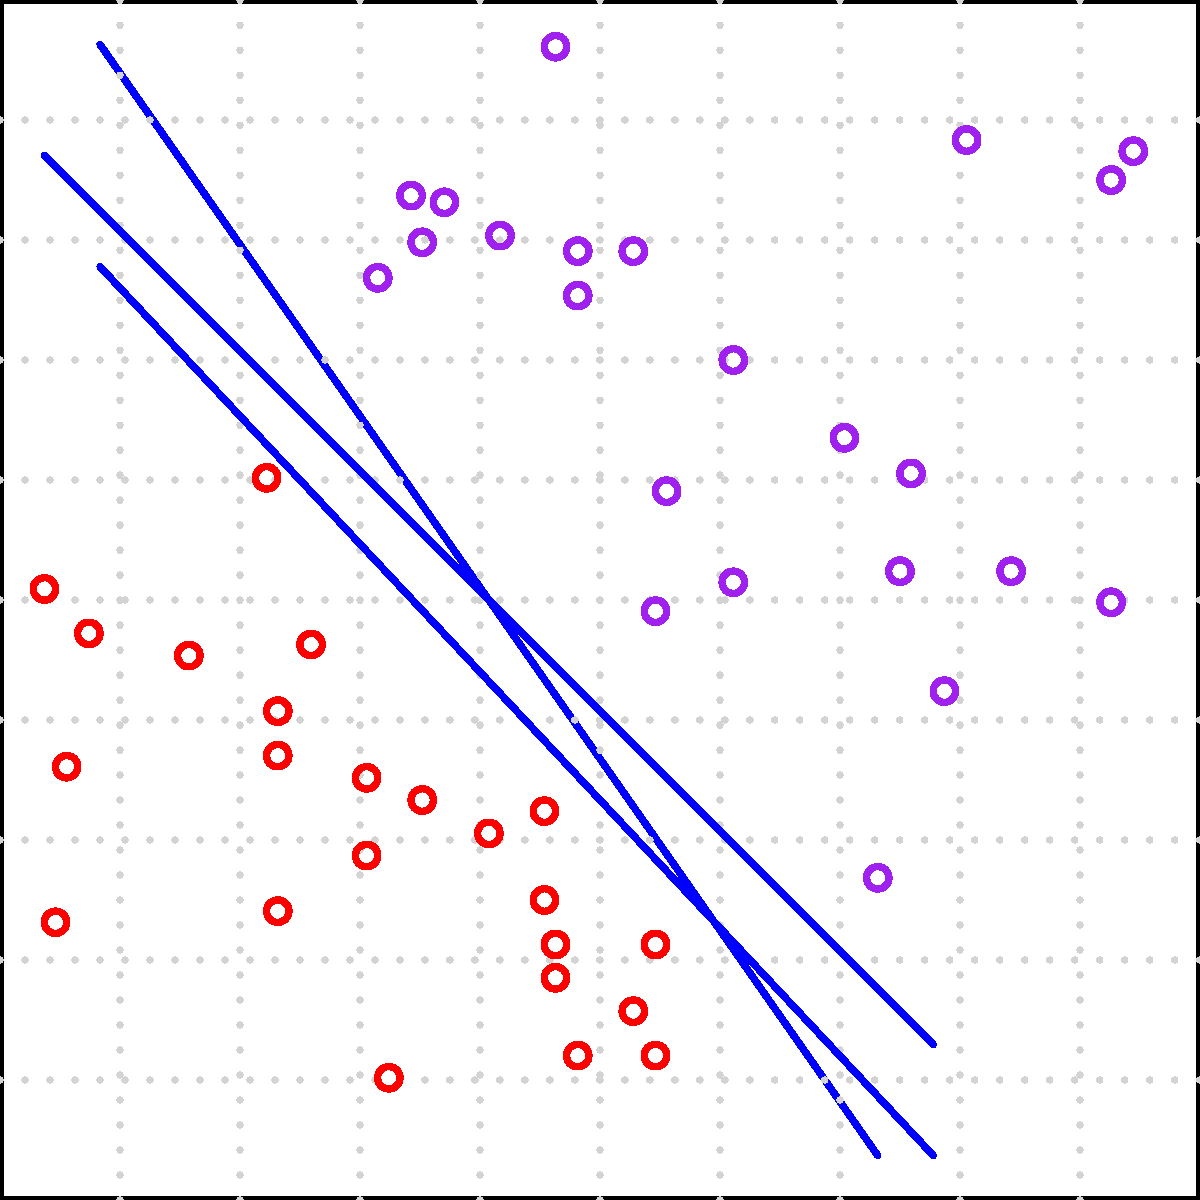
\includegraphics[scale=0.1]{./figures/empirical_risk_2.pdf}
		\end{center}
		\item We will not get a unique solution!
	\end{itemize}
\end{frame}


\begin{frame}{Regularized learning}
	\begin{itemize}
		\item Empirical risk minimization is
		\begin{itemize}
			\footnotesize
			\item ill-posed, no unique solution.
			\item overfitting, high dimensional feature space, small number of examples.
		\end{itemize}
		\item Regularization theory \citep{Evgeniou99a,Evgeniou02regularization} aims to minimize
		\begin{align*}
			\Jcal(f) = \underbrace{\Rcal_{emp}(f)}_{\text{empirical risk}} + \underbrace{\lambda\cdot\Omega(f)}_{\text{regularization}},
		\end{align*}
		the latter part controls the complexity (capacity) of the function $f$.
		\item The complexity is defined by its VC dimension as the maximum number of points that can be separated by all possible way by the set of functions.
		\item For example, the VC dimension of a hyperplane in $\RR^2$ is 3.
		\begin{center}
			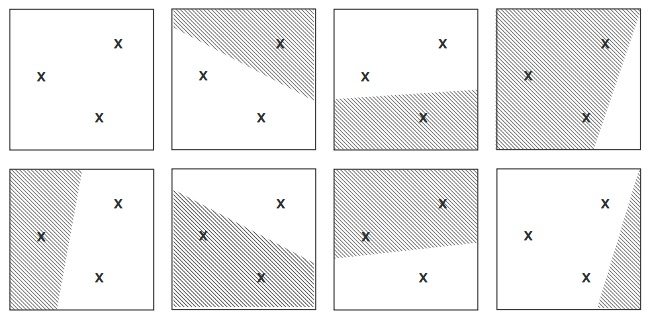
\includegraphics[scale=0.2]{./figures/vc_dimension.jpg}
		\end{center}
	\end{itemize}
\end{frame}


\begin{frame}{Regularizer}
	\begin{itemize}
		\item \citet{Vapnik92principles} shown that, the set of decision functions $f(\vx)=\ip{\vw}{\vx}+b=0$ defined on $\vXcal$ such that $||\vw||\le A$ has a VC dimension $h\le R^2A^2$.
		\item This suggests we should minimize the norm of the feature weight $||\vw||$ in order to control the complexity of the linear function class. 
		\item Popular regularizers to control the complexity
		\begin{itemize}
			\footnotesize
			\item $L_2$-norm regularizer, ridge regression \citep{Hoerl00ridge}, logistic regression \citep{Chen00}, and support vector machines \citep{Cortes95support}
			\begin{align*}
				\Omega_{L_2}(f) = ||\vw||_2=\left(\sum_{i=1}^d|\vw[i]|^2\right)^{\frac{1}{2}}.
			\end{align*}
			\item $L_1$-norm regularizer, \lasso\ \citep{Tibshirani94regression}
			\begin{align*}
				\Omega_{L_1}(f) = ||\vw||_1=\sum_{i=1}^d|\vw[i]|.
			\end{align*}
		\end{itemize}
		\item Other regularizer: graph regularizer \citep{Zhou04learning}.
	\end{itemize}
\end{frame}


\begin{frame}{Support Vector Machines}{History}
	\begin{itemize}
		\item Support Vector Machines (SVMs) was introduced by \citet{Boser92, Cortes95support}.
		\item SVM is firmly rooted from statistical learning theory \citep{Vapnik98statistical}.
		\item Good empirical performance in many applications (e.g., bioinformatics, computer vision, text classification).
		\item A large and diverse communities: e.g., machine learning, optimization, learning theory, statistics, applied computer science.
		\item Centralized website at http://www.kernel-machines.org
		\item Text books e.g.,
		\begin{itemize}
			\footnotesize
			\item An introduction to support vector machines and other kernel-based learning methods by \citet{Taylor00an}.
			\item Kernel methods for pattern analysis by \citet{Taylor04kernel}.
		\end{itemize}
	\end{itemize}
\end{frame}

\begin{frame}{Support Vector Machine}{Preliminaries}
	\begin{itemize}
		\item We focus on classification, though SVMs can do more than classification.
		\item Examples are given in pairs $(\vx,y)\in\vXcal\times\Ycal$, where $\vx\in\vXcal$ is an object and $y\in\Ycal$ is a class label.
		\item $\vXcal$ is an input space $\vXcal=\RR^d$.
		\item We consider binary classification for now, setting $\Ycal=\{-1,+1\}$.
		\item A training set of $m$ training example $\Scal=\{(\vx_i,y_i)\}_{i=1}^{m}$.
		\item We want to learn a mapping function $f: \vXcal\rightarrow\Ycal$.
		\item The mapping function is a hyperplane in the $d$-dimension feature space $\vFcal$
		\begin{align*}
			f(x) = \ip{\vw}{\vx}+b=0.
		\end{align*}
		\item For an unknown example $\vx_0$, the predicted label is given by
		\begin{align*}
			\sign(\ip{\vw}{\vx_0}+b).
		\end{align*}
	\end{itemize}
\end{frame}






\begin{frame}{Support Vector Machines}{Regularized risk minimization}
	\begin{itemize}
		\item We want to minimize a function
		\begin{align*}
			\Jcal(f) = \underbrace{\Rcal_{emp}(f)}_{\text{empirical risk}} + \underbrace{\lambda\cdot\Omega(f)}_{\text{regularization}}
		\end{align*}
		\item Use hamming loss $\ell_{hamming}$ and $L_2$ regularizer
		\begin{align*}
			\Jcal(f) = \underbrace{\frac{1}{m}\sum_{i=1}^{m}\ell_{hamming}(f(\vx_i),y_i)}_{\text{empirical risk}} + \underbrace{||\vw||^2}_{regularization}.
		\end{align*}
		\item $h_{hamming}(f(\vx_i),y_i)=1$ if $f(\vx_i)\neq y_i$, $0$ otherwise.
		\item Assume we can perfectly separate the data, we can rewrite the optimization problem as
		\begin{align*}
			\underset{\vw,b}{\minimize} &\quad \frac{1}{2}||\vw||^2 \\
			\st &\quad y_i(\ip{\vw_i}{\vx_i}+b) \ge 1, \forall i\in\{1,\cdots,m\}.
		\end{align*} 
		\item This is known as hard-margin SVMs.
	\end{itemize}
\end{frame}

\begin{frame}{Geometric interpretation}
	\begin{itemize}
		\item We are actually looking for a hyperplane with maximum margin between examples of two classes.
		\item Max-margin principle
		\begin{itemize}
			\footnotesize
			\item Robustness: small perturbation in training data does not change the classification, decision boundary only depends on the support vectors.
			\item Performance: large margin lead to low error on unseen data.
		\end{itemize}
		\item What if there is no perfect separation?
	\end{itemize}
	\begin{center}
		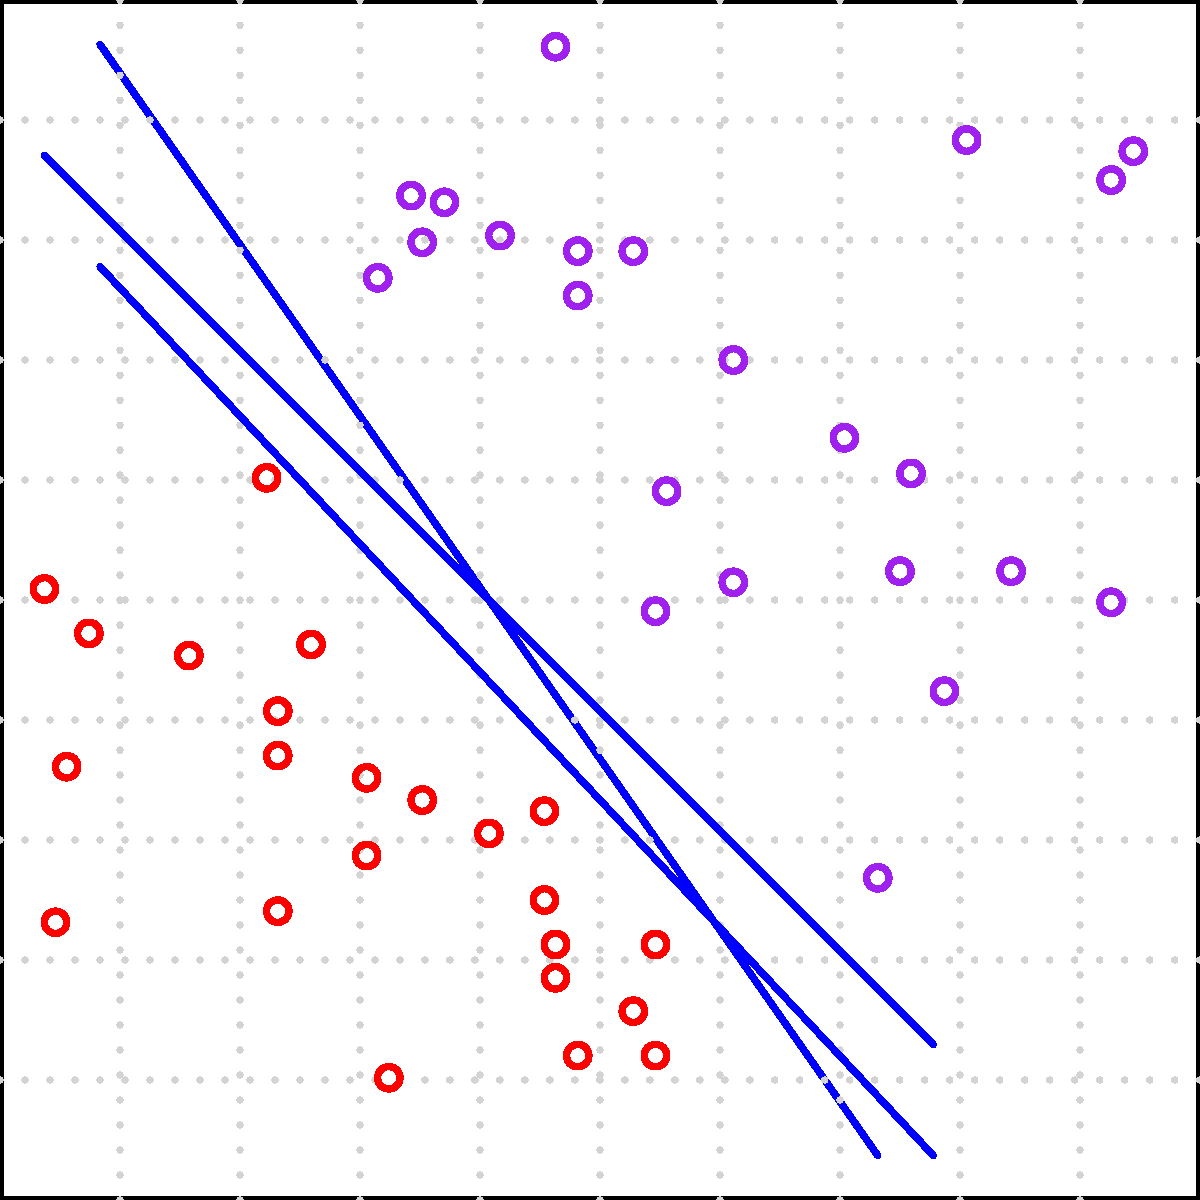
\includegraphics[scale=0.1]{./figures/empirical_risk_2.pdf}
		\text{      }
		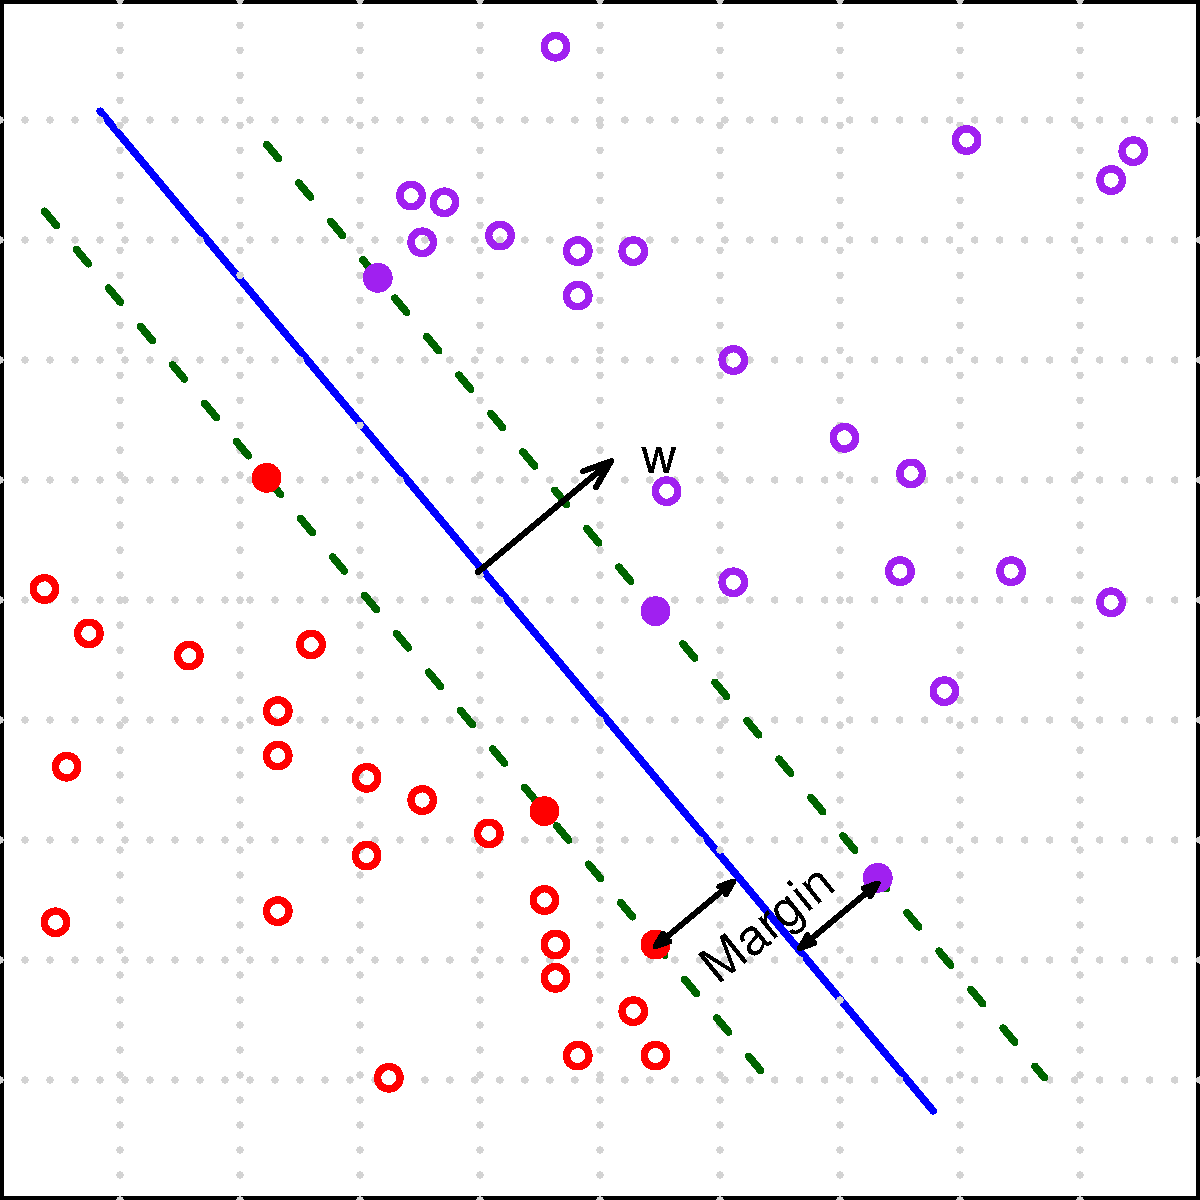
\includegraphics[scale=0.1]{./figures/maxmargin.pdf}
		\text{      }
		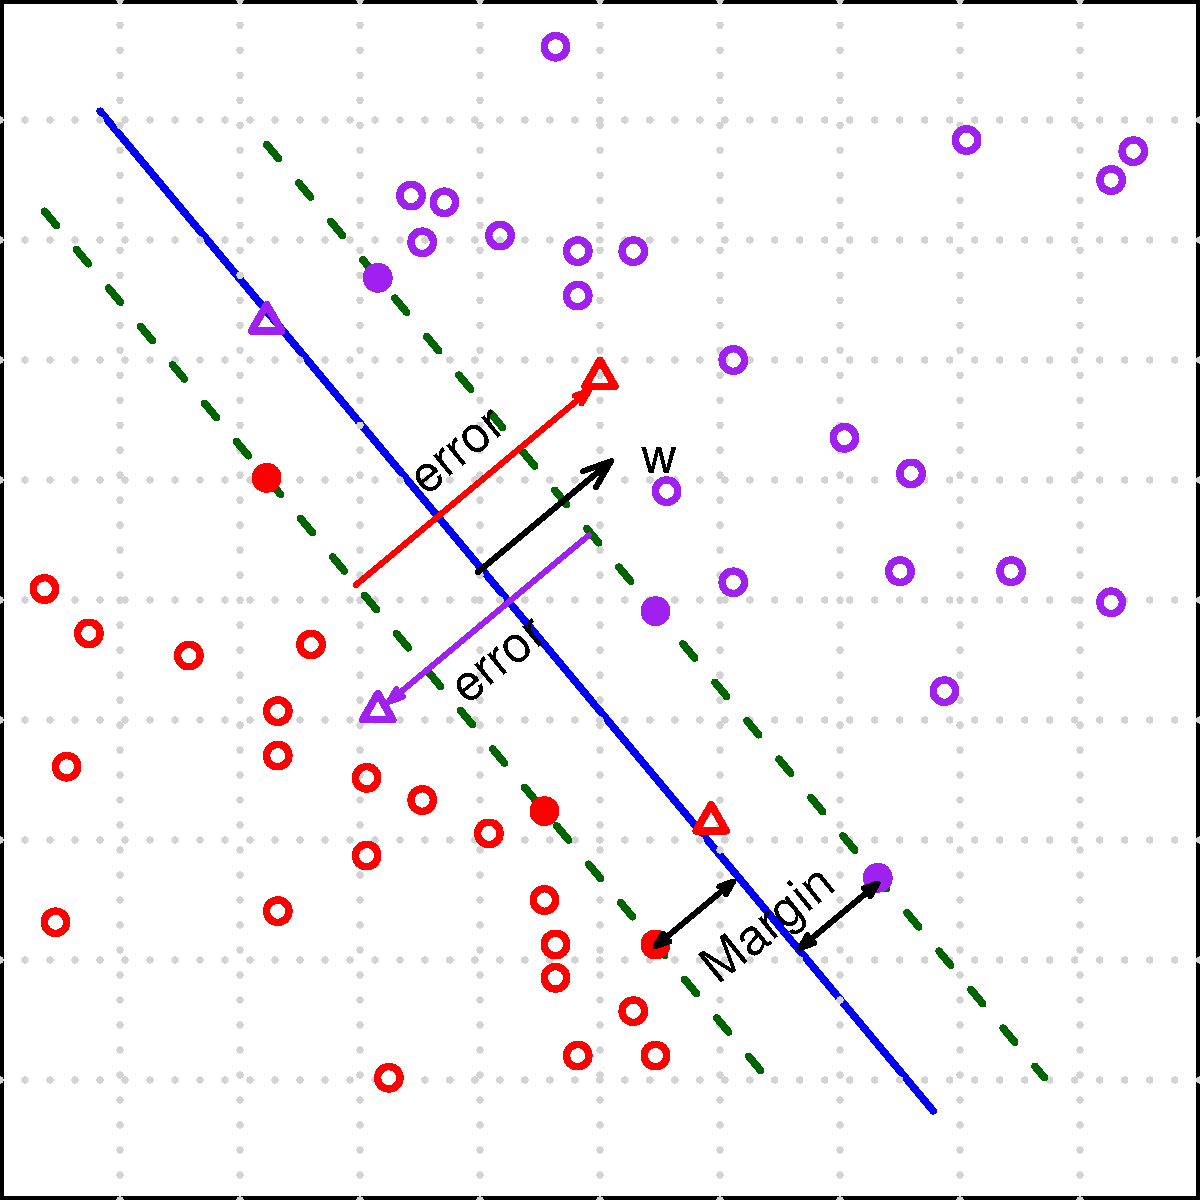
\includegraphics[scale=0.1]{./figures/soft_margin.pdf}
	\end{center}
\end{frame}

\begin{frame}{Soft-margin SVMs}
	\begin{itemize}
		\item For non-separable case, we write the optimization problem as
		\begin{align*}
			\underset{\vw,b}{\minimize} &\quad \frac{1}{2} ||\vw||^2 + C\sum_{i=1}^m\xi_i\\
            \st &\quad y_i\,(\ip{\vw}{\vx_i} + b) \ge 1-\xi_i, i\in\{1,\cdots,m\}, \xi\ge0.
		\end{align*}
		\item This is known as soft-margin SVMs.
		\item It is the same as the original objective
		\begin{align*}
			\Jcal(f) = \underbrace{\frac{1}{m}\sum_{i=1}^{m}\ell_{hinge}(f(\vx_i),y_i)}_{\text{empirical risk}} + \underbrace{||\vw||^2}_{regularization}.
		\end{align*}
		\item Hamming loss is replaced by hinge loss
		\begin{align*}
			\ell_{hinge}(f(\vx_i),y_i) = \maximize(0, 1-y_i(f(\vx_i)+b)).
		\end{align*}
	\end{itemize}
\end{frame}

\begin{frame}{Non-linear SVMs}
	\begin{itemize}
		\item Linear functions are sometimes not powerful enough.
		\item Data are not linearly separable in the original feature space.
		\item SVMs solution: map data into a richer feature space including non-linear features, then construct a hyperplane in that space.
		\item Define a input feature map
		\begin{align*}
			\vx\in\vXcal=\RR^d\overset{\varphib}{\rightarrow}\varphib(\vw)\in\vHcal =\RR^{d'}.
		\end{align*}
		\item Learn the map from $\varphib(\vx)$ to $y$
		\begin{align*}
			f(\vx) = \ip{\vw}{\varphib(\vx)} + b, \vw\in\RR^{d'}
		\end{align*}
		\begin{center}
			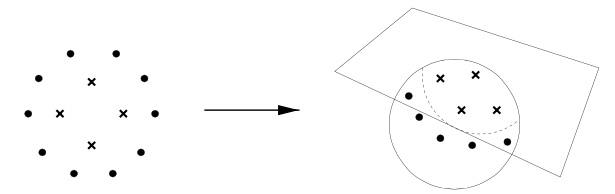
\includegraphics[scale=0.3]{./figures/nonlinearsvm.jpg}
		\end{center}
	\end{itemize}
\end{frame}


\begin{frame}{Example: polynomial feature map}
	\begin{itemize}
		\item Data points locate in two dimensional space, $\vx\in\RR^2$.
		\item We cannot separate the data point with a line.
		\item Define a feature map: 
		\begin{align*}
			\varphib:\RR^2 & \rightarrow\RR^3\\
			\vx=(x_1,x_2) & \rightarrow \varphib(\vx) \eqdef (x_1^2,\sqrt{2}x_1x_2, x_2^2)
		\end{align*}
		\item We can separate the data points with a hyperplane in the high dimensional feature space $\RR^3$.
		\begin{center}
			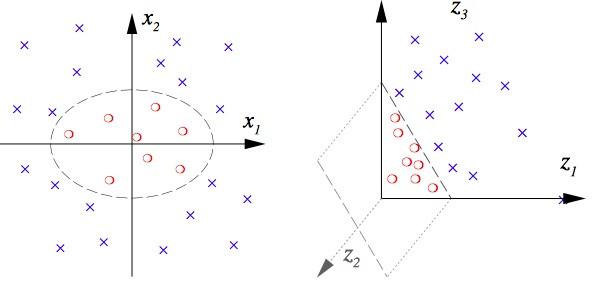
\includegraphics[scale=0.3]{./figures/polynomialfeaturemap.jpg}
		\end{center}
	\end{itemize}
\end{frame}

\begin{frame}{Kernel methods}
	\begin{itemize}
		\item Dual form of SVMs
		\begin{align*}
			\underset{\valpha}{\maximize} &\quad \sum_{i=1}^m\alpha_i - \sum_{i=1}^m\sum_{j=1}^m\alpha_i\alpha_jy_iy_j{\color{aaltoblue}\underbrace{\ip{\varphib(\vx_i)}{\varphib(\vx_j)}}_{k(\vx_i,\vx_j)}}\\
			\st &\quad 0\le\alpha_i\le C, \forall i\in\{1,\cdots,m\}.
		\end{align*}
		\item We do not need to know $\varphib(\vx_i)$ and $\varphib(\vx_j)$, we only need the results of the inner product $\ip{\varphib(\vx_i)}{\varphib(\vx_j)}$.
		\item Kernel is a function $k:\vXcal\times\vXcal\rightarrow\RR$
		\begin{align*}
			k(\vx_i,\vx_j) = \ip{\varphib(\vx_i)}{\varphib(\vx_j)},
		\end{align*}
		$\varphib:\vXcal\rightarrow\vHcal$ is the input feature map.
		\item Kernel function is used to make (implicit) nonlinear feature map.
		\item Kernel function can be evaluated in original space $\vXcal$ without working explicitly in high the dimensional space $\vHcal$.
	\end{itemize}
\end{frame}

\begin{frame}{An example of kernel function}
	\begin{itemize}
		\item Degree two polynomial kernel
		\begin{align*}
			k(\vx,\vz) = (\ip{\vx}{\vz})^2, \vx,\vz\in\RR^2.
		\end{align*} 
		\item Evaluate kernel function in original feature space $\RR^2$
		\begin{align*}
			k(\vx,\vz) &= (\ip{(x_1,x_2)}{(z_1,z_2)})^2 \\
			&= x_1^2z_1^2+x_2^2z_2^2+2x_1x_2z_1z_2 
		\end{align*}
		\item Explicit feature map
		\begin{align*}
			\vx=(x_1,x_2)\in\RR^2\overset{\varphib}{\rightarrow}\varphib(\vx)=(x_1^2,\sqrt{2}x_1x_2,x_2^2)\in\RR^3\\
			\vz=(z_1,z_2)\in\RR^2\overset{\varphib}{\rightarrow}\varphib(\vz)=(z_1^2,\sqrt{2}z_1z_2,z_2^2)\in\RR^3
		\end{align*}
		\item Evaluate kernel function with explicit feature map
		\begin{align*}
			\ip{\varphib(\vx)}{\varphib(\vz)} 
			&= \ip{(x_1^2,\sqrt{2}x_1x_2,x_2^2)}{(z_1^2,\sqrt{2}z_1z_2,z_2^2)}\\
			&= x_1^2z_1^2+x_2^2z_2^2+2x_1x_2z_1z_2
		\end{align*}
		
	\end{itemize}
\end{frame}


\begin{frame}{Popular kernels}
	\begin{itemize}
		\item Linear kernel
		\begin{align*}
			k_{linear}(\vx_i,\vx_j) = \ip{\vx_i}{\vx_j}.
		\end{align*}
		\item Polynomial kernel
		\begin{align*}
			k_{poly}(\vx_i,\vx_j) = (\ip{\vx_i}{\vx_j} + b)^d.
		\end{align*}
		\item Gaussian kernel
		\begin{align*}
			k_{gaussian}(\vx_i,\vx_j) = \exp\left(\frac{||\vx_i-\vx_j||^2}{2\delta^2}\right).
		\end{align*}
	\end{itemize}
\end{frame}


\begin{frame}{SVMs Softwares}
	\begin{itemize}
		\item LibSVM, in \cpp, by \citet{Chang11libsvm}
		\item SVMLight, in \ccc, by \citet{Joachims98making}
		\item Torch (http://bengio.abracadoudou.com/SVMTorch.html)
		\item Spider (http://people.kyb.tuebingen.mpg.de/spider/)
		\item Weka (http://www.cs.waikato.ac.nz/ml/weka/index.html)
	\end{itemize}
\end{frame}

\begin{frame}{Molecular classification}
	\begin{itemize}
		\item
	\end{itemize}
\end{frame}

\begin{frame}{Multi-task classification}
	\begin{itemize}
		\item 
	\end{itemize}
\end{frame}

\begin{frame}{Max-margin conditional random field}{Preliminaries}
	\begin{itemize}
		\item Training examples come in pairs $(\vx,\vy)\in\vXcal\times\vYcal$ sampled from some unknown joint distribution $P(\vx,\vy)$.
		\item $\vx\in\vXcal$ is an instant from input domain $\vXcal$ (e.g., a document, a molecule, a picture).
		\item $\vy=(y_1,\cdots,y_k)\in\vYcal$ is a vector of labels from output domain (e.g., categories of a documents, potentials of a molecules, annotations of a picture).
		\item The output domain $\vYcal=\Ycal_1\times\cdots\times\Ycal_k$, $\Ycal_j=\{-1,+1\}$ and $\vYcal=\{-1,+1\}^k$.
		\item $\vy$ is called a multilabel, $y_i$ is called a microlabel of the multilabel.
		\item We are given a set of training examples $S=\{(\vx_i,\vy_i)\}_{i=1}^m$.
		\item A pair $(\vx_i,\vy)$ is called pseudo example, $\vy\in\vYcal$.
		\item The goal is to obtain a function $f:\vXcal\rightarrow\vYcal$.
		\begin{table}
		\footnotesize
		\begin{tabular}{p{1cm}p{1cm}p{10cm}}
        \multirow{3}{*}{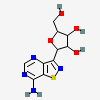
\includegraphics[scale = 0.3]{./figures/mol1.png}} & 
			& \\ 
		& $\rightarrow$	& $\vy=(y_1,y_2,y_3,y_4)=(+1,-1,+1,+1)$ \\
		&	& \\ 
        \end{tabular}
        \end{table}
	\end{itemize}
\end{frame}

\begin{frame}{Output graph and feature maps}
	\begin{itemize}
		\item Observe an output graph $G=(E,V)$, a vertex $v_i\in V$ correspond to a microlabel $y_i$, an edge $(v_i,v_j)\in E$ correspond to the pairwise correlation of the microlabel $y_i$ and $y_j$.
		\begin{center}
			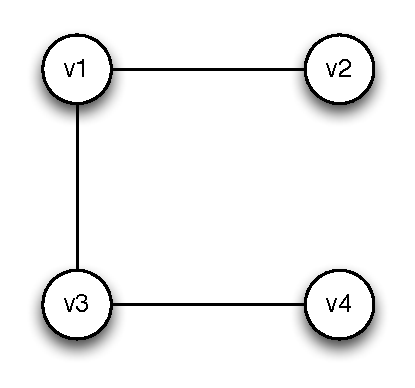
\includegraphics[scale=0.3]{./figures/outputgraph.pdf}
		\end{center}
		\item $\varphib(\vx)$ is the  input feature map, $\varphib(\vx)\in\RR^d$.
		\item $\psib(\vy)$ is the output feature map that maps the multilabel $\vy$ into a set of edges and labels, $\psib(\vy)\in\RR^{4|E|}$.
		\begin{align*}
			\vy&=(y_1,y_2,y_3,y_4)=(+1,-1,+1,+1)\\
			\psib(\vy) &= ( \underbrace{\underbrace{0}_{--}, \underbrace{0}_{-+}, \underbrace{1}_{+-}, \underbrace{0}_{++},}_{(v_1,v_3)} 
			\underbrace{\underbrace{0}_{--}, \underbrace{0}_{-+}, \underbrace{0}_{+-}, \underbrace{1}_{++},}_{(v_1,v_2)}
			\underbrace{\underbrace{0}_{--}, \underbrace{0}_{-+}, \underbrace{0}_{+-}, \underbrace{1}_{++}}_{(v_3,v_4)})
		\end{align*}
	\end{itemize}
\end{frame}


\begin{frame}{Compatibility score}
	\begin{itemize}
		\item Joint feature map put input and output feature into a joint feature space
		\begin{align*}
			\phib(\vx,\vy) = \varphi(\vx)\otimes\psi(\vy) = (\varphib(\vx)[i]\,\psib(\vy)[j])_{i,j},
		\end{align*} 
			$\otimes$ is the Kronecker product. $\phib(\vx,\vy)\in\RR^{d\times4|E|}$
		\begin{center}
			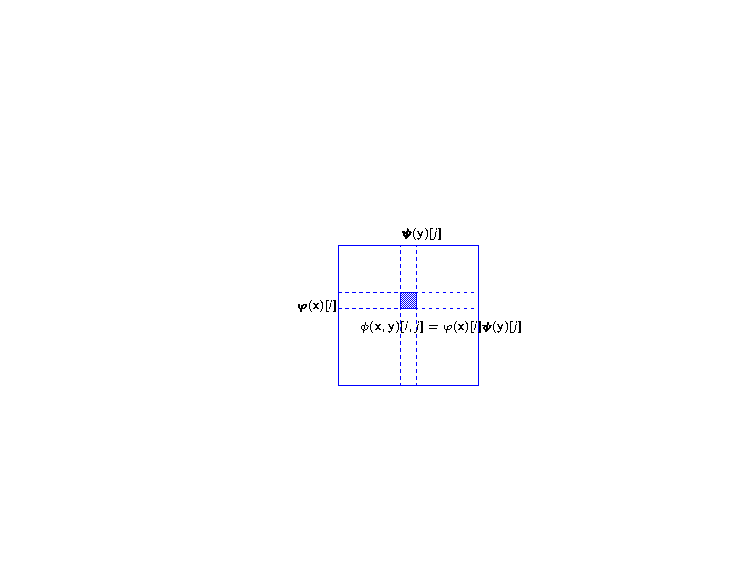
\includegraphics[scale = 1]{./figures/tensor_label.pdf}	
			\text{     }
			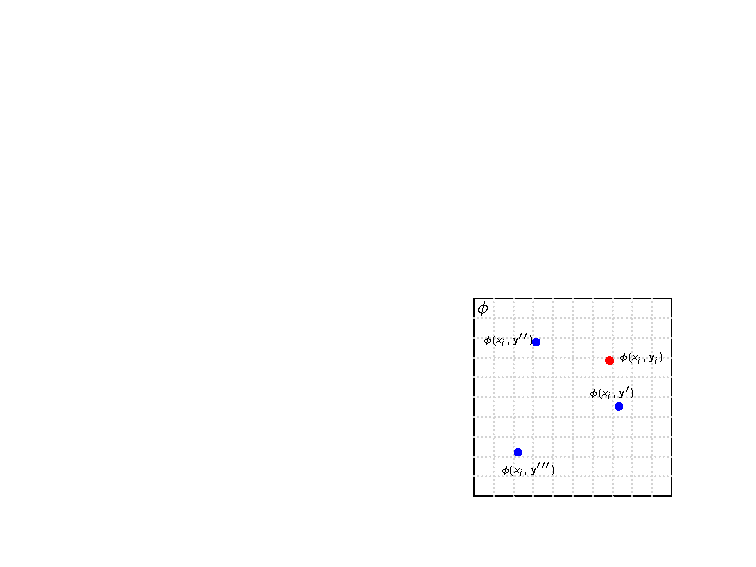
\includegraphics[scale = 0.7]{./figures/jointfeaturespace.pdf}	
		\end{center}
		% \begin{center}
		% 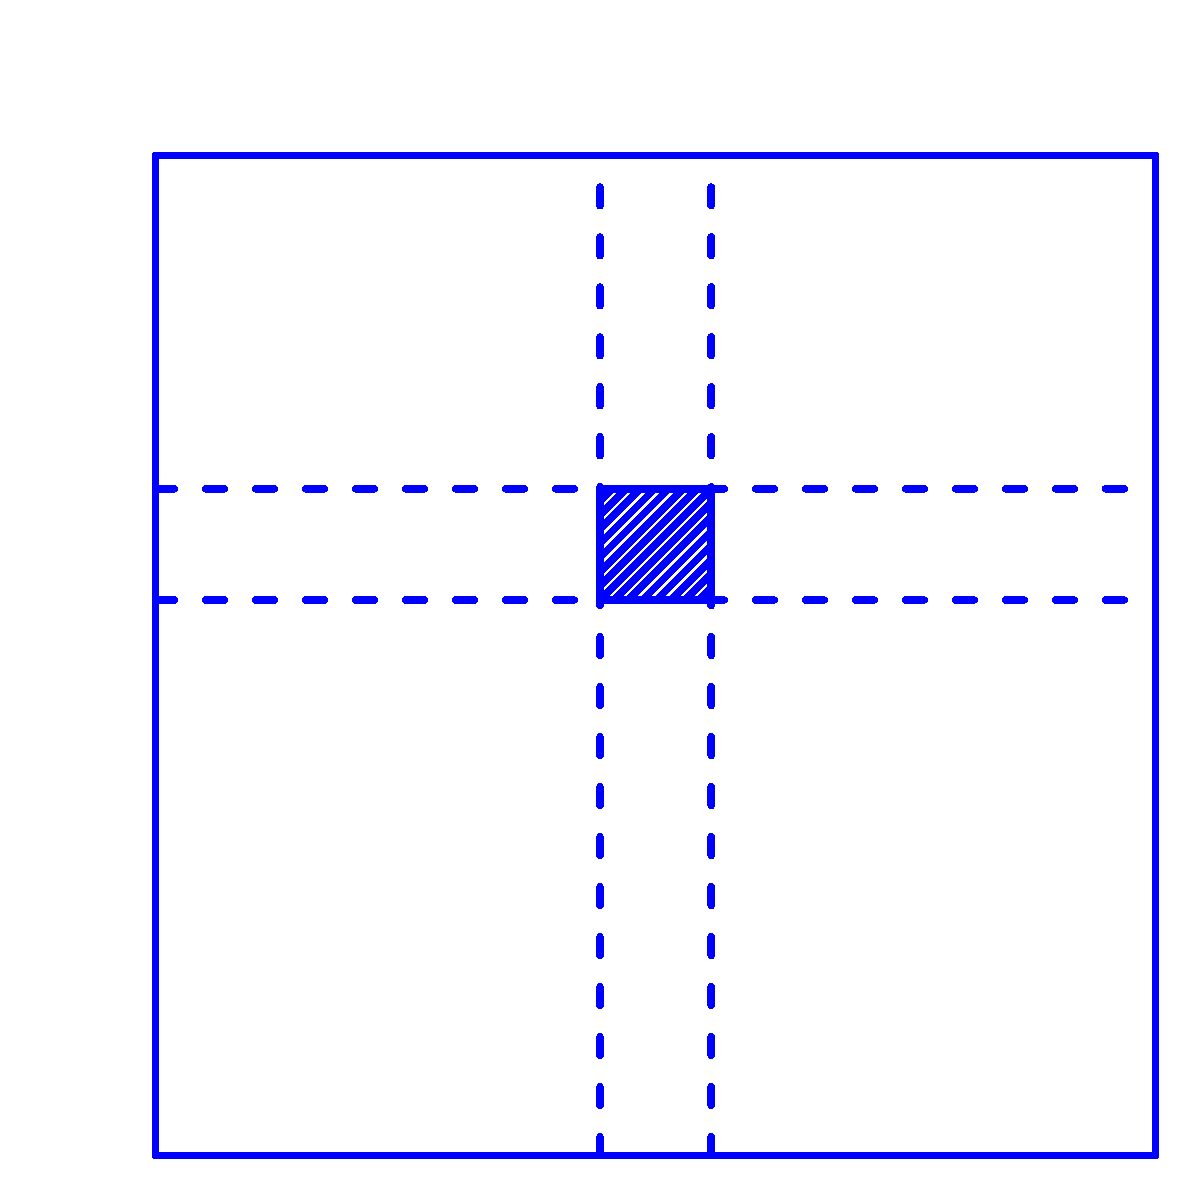
\includegraphics[scale = 0.14]{./figures/tensor.pdf}
		% \put(-90,40){\tiny $\varphib(\vx)[i]$}
		% \put(-40,75){\tiny $\psib(\vy)[j]$}
		% \put(-60,30){\tiny $\phi(\vx,\vy)[i,j] = \varphi(\vx)[i]\psib(\vy)[j]$}
		% \end{center}
		\item For now we assume we already have optimal $\vw$, compatibility score will assign high value to $(\vx_i,\vy_i)$ compared to $(\vx_i,\vy),\vy\in\vYcal/\vy_i$
		\begin{align*}
			F(\vx_i,\vy_i;\vw) = \ip{\vw}{\phib(\vx_i,\vy_i)}.
		\end{align*}
		\item Prediction is by solving the $\argmax$ in exponential space $|\vYcal|=2^k$
		\begin{align*}
			\vy^*= \underset{\vy\in\vYcal}{\argmax} \, F(\vx,\vy) =  \underset{\vy\in\vYcal}{\argmax} \,\ip{\vw}{\phib(\vx,\vy)}.
		\end{align*}
		\item 
	\end{itemize}
\end{frame}

\begin{frame}{Obtain $\vw$ by regularized learning}
	\begin{itemize}
		\item $L_2$ norm regularization on $\vw$, $\Omega(f) = ||\vw||^2$.
		\item Risk term
		\begin{itemize}
			\footnotesize
			\item $f$ will not make mistake if
			\begin{align*}
				F(\vx_i,\vy_i) - F(\vx_i,\vy) \ge 0, \forall \vy\in\vYcal/\vy_i, i\in\{1,\cdots,m\}.
			\end{align*}
			\item We only have to evaluate the score of best incorrect label 
			\begin{align*}
				F(\vx_i,\vy_i) - \underset{\vy\in\vYcal/\vy_i}F(\vx_i,\vy) \ge 0, \forall i\in\{1,\cdots,m\}.
			\end{align*}
		\end{itemize}
		
		\item The \mmcrf\ optimization problem
		\begin{align*}
			\underset{\vw,\vxi}{\minimize} &\quad \underbrace{\frac{1}{2}||\vw||^2}_{\text{regularization}} + \underbrace{C\sum_{i=1}^m\xi_i}_{\text{risk}}\\
			\st &\quad F(\vx_i,\vy_i) - \underset{\vy\in\vYcal/\vy_i}{\maximize}F(\vx_i,\vy) \ge \ell(\vy_i,\vy) + \xi_i,\\
			&\quad \xi_i\ge0, \forall i\in\{1,\cdots,m\}.
		\end{align*}
	\end{itemize}
\end{frame}


\begin{frame}[allowframebreaks]{Bibliography}
%\bibliographystyle{plain}
\bibliographystyle{apalike}
 \bibliography{dissertation}
\end{frame}

}
\end{document}
%%%%%%%%%%%%%%%%%%%%%%%%%%%%%%%%%%%%%%%%%%%%%%%%%%%%%%%%%%%%%%%%%%%%%%%%%%%%%%%%%%%%%%%%%%%%%






